% set the document type and the font size
\documentclass[12pt]{article}

% use Spanish package
\usepackage[spanish]{babel}

% set UTF-8 codification
\usepackage[utf8]{inputenc}

% insert images
\usepackage{graphicx}
\graphicspath{ {images/} }

% captions without name
\usepackage{caption}

% insert graphical tree
\usepackage{tikz}
\usepackage{tikz-qtree}

% no equation numeration
\usepackage{amsmath}

% use tables
\usepackage{booktabs}

% use special superindex
\usepackage{stackrel}

% overline words
\usepackage{soul}

% set contents to page using [H]
\usepackage{float}

% create the title
\title{\textbf{Sistemas Digitales}}
\date{2017-18}
\author{Diego Enrique Fontán, CosasDePuma}

\begin{document}
	% no page numbers
	\pagenumbering{gobble}

	% title
	\maketitle
	\newpage
	
	% table of contents
	\tableofcontents
	\newpage
	
	% arabic numeration
	\pagenumbering{arabic}
	
	\section{Introducción a los Sistemas Digitales}
	
		\vfill
	
		\subsection{Tipos de señales}
			
			Tipos de señales que nos podemos encontrar en relación a los valores que pueden tomar:\\
		
			- \textbf{Señales analógicas:} Pueden tomar infinitos valores distintos a lo largo del tiempo.\\
		
			- \textbf{Señales digitales:} Sólo pueden tomar un número finito de valores distintos a lo largo del tiempo.\\
				
			\begin{figure}[H]
			\centering
			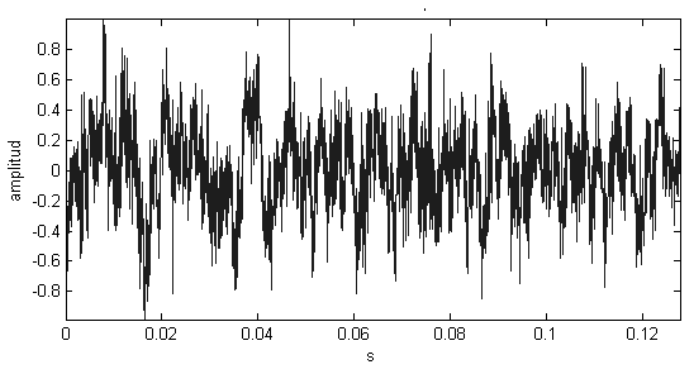
\includegraphics[width=150px,height=100px]{analogic}
			\caption{Ejemplo de señal analógica}
			\end{figure}
		
			\begin{figure}[H]
			\centering
			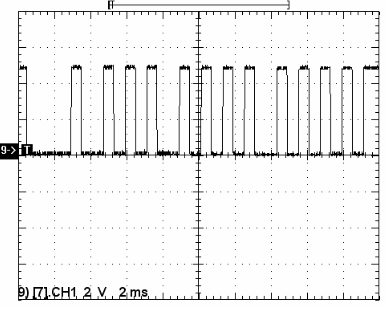
\includegraphics[width=140px,height=100px]{digital}
			\caption{Ejemplo de señal digital}
			\end{figure}
			
			\newpage
	
		\subsection{Señales binarias}
	
			Las señales binarias son un caso particular de las señales digitales.\\
			
			Se caracterizan porque sólo pueden tomar dos valores distintos a lo largo del tiempo.\\
	
			Los sistemas electrónicos digitales que se utilizan hoy en día operan con señales binarias.\\
			
			Por lo tanto, según el valor que tome la señal en cada momento, se pueden determinar dos estados diferentes que posteriormente se emparejarán a números binarios.\\
			
			\begin{figure}[H]
			\centering
			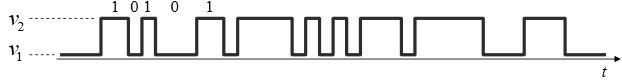
\includegraphics[width=250px,height=50px]{binary}
			\caption{Ejemplo de señal binaria}
			\end{figure}
			
			El que se denomine a los sistemas que utilizan estas señales como \textit{sistemas digitales} en vez de \textit{sitemas binarios} se debe a que, en general, procesan valores digitales, los cuales se codifican mediante combinaciones de valores binarios para que puedan ser tratados.\\
			
		\subsection{Ventajas de los sistemas digitales}
		
			Las ventajas que tienen los sistemas digitales respecto a los analógicos son, entre otras:\\
			
			- Son más fáciles de diseñar.
			
			- Son menos sensibles a agentes externos (como a las interferencias).
			
			- Permiten almacenar y operar con grandes cantidades de información de forma rápida y segura.
			
			
			
			\newpage
			
	\section{Sistemas de numeración y códigos binarios}
	
		\vfill
		
		Un sistema de numeración no es más que un método que se usa para representar cantidades de forma simbólica, siguiendo ciertas normas y convenios.\\
		
		Un número es una representación mediante símbolos de una cantidad dada.\\
		
		Una misma cantidad puede ser representada mediante un número distinto en función del sistema de numeración que se considere.\\
		
		Por ejemplo:\\
		
		\[
		12_{10} = C_{16} = 14_{8} = 1100_{2}
		\]
	
		Los sistemas de numeración sólamente expresan el módulo, magnitud o valor absoluto de una cantidad, nunca si es positiva o negativa.\\
		
		Hoy en día utilizamos sistemas de numeración posicionales, caracterizados por:\\
		
		- Las cantidades se representan mediante una sucesión ordenada de números a ambos lados de un símbolo de referencia (punto, coma...)\\
		
		\begin{figure}[H]
			\centering
			\Tree [.Cantidad  [.3735928559 entera ] [., símbolo ] [.129152485 fraccionaria ] ]
		\end{figure}
		
		- Cada dígito tiene asociado un \textbf{peso} cuyo valor depende de la \textbf{base} y de la \textbf{posición} que ocupe el dígito.\\
		
		\newpage
			
		\subsection{Sistemas de numeración}
		
			Un sistema de numeración de base \textbf{b} utiliza hasta \textbf{b} símbolo para representar diferentes cantidades.\\
			
			La base de un sistema de numeracíon también se denomina \textit{raíz} o \textit{módulo}.\\
			
			\begin{table}[H]
				\centering
				\begin{tabular}{c|c}
					Sistema de numeración & Símbolos utilizados\\
					\midrule
					Binario (base = 2) & 0, 1\\
					Ternario (base = 3) & 0, 1, 2\\
					Octal (base = 8) & 0, 1, 3, 4, 5, 6, 7\\
					Decimal (base = 10) & 0, 1, 2, 3, 4, 5, 6, 7, 8, 9\\
					Hexadecimal (base = 16) & 0, 1, 2, 3, 4, 5, 6, 7, 8, 9, A, B, C, D, E, F\\
				\end{tabular}
				\caption{Símbolos usados según el sistema de numeración utilizado}
			\end{table}
			
			Como hemos visto, una misma cantidad se puede representar de diferentes maneras, según la base que utilicemos. La tabla de equivalencias entre los diferentes sistemas de numeración más utilizados sería la siguiente:\\
			
			\begin{table}[H]
				\centering
				\label{table:con}
				\begin{tabular}{c|c|c|c||c|c|c|c}
					Binario & Octal & Decimal & Hexadec. & Binario & Octal & Decimal & Hexadec. \\
					\toprule
					0000 & 00 & 00 & 0 & 1000 & 10 & 08 & 8 \\
					0001 & 01 & 01 & 1 & 1001 & 11 & 09 & 9 \\
					0010 & 02 & 02 & 2 & 1010 & 12 & 10 & A \\
					0011 & 03 & 03 & 3 & 1011 & 13 & 11 & B \\
					0100 & 04 & 04 & 4 & 1100 & 14 & 12 & C \\
					0101 & 05 & 05 & 5 & 1101 & 15 & 13 & D \\
					0110 & 06 & 06 & 6 &1110 & 16 & 14 & E \\
					0111 & 07 & 07 & 7 & 1111 & 17 & 15 & F \\
					\bottomrule					
				\end{tabular}
			\end{table}
			
			\newpage
			      
	\subsection{Peso numérico según la base y posición}
		
			Las posiciones y los pesos asociados a cada uno de los dígitos de una cantidad guardan la siguiente relación:
			
			\begin{equation}
				\notag
				\overbrace{\underbrace{{a}_{n-1}^{{b}^{n-1}}\ {a}_{n-2}^{{b}^{n-2}}\ ...\ {a}_{1}^{b}\ {a}_{0}^{1}}_{parte\ entera}\ ,\ \underbrace{{a}_{-1}^{{b}^{-1}}\ {a}_{-2}^{{b}^{-2}}\ ...\ {a}_{-(m-1)}^{{b}^{-(m-1)}}\ {a}_{-m}^{{b}^{-m}}}_{parte\ fraccionaria}}^{pesos}
			\end{equation}\\
			
			Veamos los pesos asociados a la base decimal:
			
			\begin{equation}
				\notag
				\stackbin{10000}{{10}^{4}} ~ \stackbin{1000}{{10}^{3}} ~ \stackbin{100}{{10}^{2}} ~ \stackbin{10}{{10}^{1}} ~ \stackbin{1}{{10}^{0}} ~ \stackbin{0.1}{{10}^{-1}} ~ \stackbin{0.01}{{10}^{-2}} ~ \stackbin{0.001}{{10}^{-3}} ~ \stackbin{0.0001}{{10}^{-4}}
			\end{equation}\\
			
			También es importante poder identificar rápidamente los pesos asociados a la base binaria:\\
			
			\begin{equation}
				\notag
				\stackbin{256}{{2}^{8}} ~ \stackbin{128}{{2}^{7}} ~ \stackbin{64}{{2}^{6}} ~ \stackbin{32}{{2}^{5}} ~ \stackbin{16}{{2}^{4}} ~ \stackbin{8}{{2}^{3}} ~ \stackbin{4}{{2}^{2}} ~ \stackbin{2}{{2}^{1}} ~ \stackbin{1}{{2}^{0}} ~ \stackbin{0.5}{{2}^{-1}} ~ \stackbin{0.25}{{2}^{-2}} ~ \stackbin{0.125}{{2}^{-3}} ~ \stackbin{0.0625}{{2}^{-4}}
			\end{equation}
			
		\subsection{Conversión entre bases}
		
			\subsubsection{A base decimal}
		
				Para pasar una cantidad \underline{en una base cualquiera a base decimal}, se utiliza la fórmula determinada como \textbf{polinomio característico}:\\
			
				\begin{equation}
					\notag
					{N}_{b} = \sum_{i=-m}^{i=n-1}{a}_{i}{b}^{i} = \underbrace{{a}_{n-1}{b}^{n-1} + ... + {a}_{1}{b}^{1} + {a}_{0}{b}^{0}}_{parte\ entera} + \underbrace{{a}_{-1}{b}^{-1} + {a}_{-2}{b}^{-2} + ... + {a}_{-m}{b}^{-m}}_{parte\ fraccionaria}
				\end{equation}
			
				\newpage
				
			\subsubsection{De decimal a binario}
			
					- \underline{\textbf{Método Teórico:}} La representación de la parte entera de un número decimal se calcula como sucesivas divisiones entre 2 hasta obtener un coeficiente menor que dos. La solución está formada por los restos de las divisiones \underline{en orden inverso al que se han ido generando}.\\
					
						\begin{table}[H]
							\centering
							\begin{tabular}{cccc}
								Dividendo & Divisor & Cociente & \textbf{Resto} \\
								\toprule
								12 & 2 & 6 & \textbf{0} \\
								6 & 2 & 3 & \textbf{0} \\
								3 & 2 & 1 & \textbf{1} \\
								\midrule
								1 & 2 & 0 & \textbf{1} \\
							\end{tabular}
							\caption*{12 de decimal a binario}
						\end{table}
						
						Como los restos se leen en el orden inverso al obtenido, $12_{10}$ en decimal es $1100_{2}$ en binario.\\
						
						Para determinar la representación de una parte fraccionaria, se realizan multiplicaciones por 2 hasta obtener el número de dígitos deseados o hasta que la parte fraccionaria de la conversión sea cero (exacta).\\
						
						La representación en binario de la parte fraccionaria está formada por los valores enteros de los resultados leídos \underline{en el orden en el que se obtienen}.
						
						\begin{table}[H]
							\centering
							\begin{tabular}{ccc}
								0,2017 & x 2 = & \textbf{0},4034 \\
								0,4034 & x 2 = & \textbf{0},8068 \\
								0,8068 & x 2 = & \textbf{1},6136 \\
								0,6136 & x 2 = & \textbf{1},2257 \\
								0,2257 & x 2 = & \textbf{0},4544 \\
								0,4544 & x 2 = & \textbf{0},9088 \\
								0,9088 & x 2 = & \textbf{1},8176 \\
								& \vdots & \\
							\end{tabular}
							\caption*{0,2017 de decimal a binario}						 
						\end{table}
						
						\newpage

						Como la parte entera se lee en el orden obtenido, $0.2017_{10}$ en decimal es $0011001_{2}$ en binario con 7 bits de precisión.\\
						
						Si lo que queremos es representar un número con parte entera y parte fraccionaria, seguiremos los pasos descritos anteriormente y los uniremos en un mismo número.\\
						
						De esta forma:
						
						\begin{equation}
							\notag
							12,2017_{10} = 1100,0011001_{2}
						\end{equation}\\
						
				- \underline{\textbf{Método práctico:}} Sabiendo los pesos de la base binaria, pondremos (de derecha a izquierda) un 1 en la posición que nos de una cantidad menor o igual al número que estamos buscando y un 0 en el que nos de un valor mayor al deseado.\\
						
						\begin{table}[H]
							\centering
							\caption*{\underline{90,25 de decimal a binario}}
							\begin{tabular}{ccccccc|cccc||c}
								\toprule
								64 & 32 & 16 & 8 & 4 & 2 & 1 & 0.5 & 0.25 & 0.125 & 0.0625 & Decimal acumulado \\
								\midrule
								0 & 0 & 0 & 0 & 0 & 0 & 0 & 0 & 0 & 0 & 0 & 00,00 \\
								\textbf{1} & 0 & 0 & 0 & 0 & 0 & 0 & 0 & 0 & 0 & 0 & 64,00 \\
								\st{1}&\st{\textbf{1}}&\st{0}&\st{0}&\st{0}&\st{0}&\st{0}&\st{0}&\st{0}&\st{0}&\st{0}&\st{96,00} \\
								1 & 0 & \textbf{1} & 0 & 0 & 0 & 0 & 0 & 0 & 0 & 0 & 80,00 \\
								1 & 0 & 1 & \textbf{1} & 0 & 0 & 0 & 0 & 0 & 0 & 0 & 88,00 \\
								\st{1}&\st{0}&\st{1}&\st{1}&\st{\textbf{1}}&\st{0}&\st{0}&\st{0}&\st{0}&\st{0}&\st{0}&\st{92,00} \\
								1 & 0 & 1 & 1 & 0 & \textbf{1} & 0 & 0 & 0 & 0 & 0 & 90,00 \\
								\st{1}&\st{0}&\st{1}&\st{1}&\st{0}&\st{1}&\st{\textbf{1}}&\st{0}&\st{0}&\st{0}&\st{0}&\st{91,00} \\
								\st{1}&\st{0}&\st{1}&\st{1}&\st{0}&\st{1}&\st{0}&\st{\textbf{1}}&\st{0}&\st{0}&\st{0}&\st{90,50} \\
								1 & 0 & 1 & 1 & 0 & 1 & 0 & 0 & \textbf{1} & 0 & 0 & \textbf{90,25} \\
								\bottomrule
							\end{tabular}
						\end{table}
						
						De esta forma obtenemos que:
						
						\begin{equation}
							\notag
							90.25_{10} = 1011010,01_{2}
						\end{equation}
					
						\newpage
						
			\subsubsection{De decimal a cualquier base}
			
				Para ello tendremos que seguir los pasos descritos en el apartado anterior pero cambiando el operando de las multiplicaciones y divisiones. En vez de utilizar un 2, utilizaremos el módulo de nuestra base. Por ejemplo:\\
				
				\begin{table}[H]
					\centering
					\begin{tabular}{cccl}
						Dividendo & Divisor & Cociente & \textbf{Resto} \\
						\toprule
						2894 & 16 & 180 & \textbf{E} (14)\\
						180 & 16 & 11 & \textbf{4} \\
						\midrule
						11 & 16 & 0 & \textbf{B} (11) \\
					\end{tabular}
					\caption*{$2894_{10}$ es lo mismo que $B4E_{16}$}
				\end{table}
				
				Lo mismo ocurre si nos sabemos los pesos, aunque a causa de tener más símbolos que 0 y 1, este método se vuelve inviable:\\
				
				\begin{table}[H]
							\centering
							\caption*{\underline{545 de decimal a octal}}
							\begin{tabular}{cccc||c}
								\toprule
								512 & 64 & 8 & 1 & Decimal acumulado \\
								\midrule
								0 & 0 & 0 & 0 & 000 \\
								\textbf{1} & 0 & 0 & 0 & 512 \\
								\st{1}&\st{\textbf{1}}&\st{0}&\st{0}&\st{576} \\
								\st{1}&\st{0}&\st{\textbf{7}}&\st{0}&\st{568} \\
								\st{1}&\st{0}&\st{\textbf{6}}&\st{0}&\st{560} \\
								\st{1}&\st{0}&\st{\textbf{5}}&\st{0}&\st{552} \\
								1 & 0 & \textbf{4} & 0 & 544\\
								1 & 0 & 4 & \textbf{1} & \textbf{545}\\
								\bottomrule
							\end{tabular}
							\caption*{$545_{10}$ es equivalente a $1041_8$}
						\end{table}
						
						\newpage
						
			\subsection{De binario a octal o hexadecimal}
				
				Dado que tanto binario, cuaternario, octal, hexadecimal... son bases que tienen como módulo una potencia de 2, se da entre ellas una propiedad que permite realizar cambios de una manera mucho más cómoda y fluída.\\
				
				Por ejemplo, si queremos pasar de binario a octal, deberemos separar desde la coma grupos de 3 dígitos binarios y rellenar aquellos que sobren con ceros.\\
				
				Sea el número $10 111 110.1_2$:\\
				
				\begin{equation}
					\notag
					\underbrace{\textbf{0}10} \underbrace{111} \underbrace{110} ~,~ \underbrace{1\textbf{0}\textbf{0}}
				\end{equation}\\
				
				Posteriormente sustituímos cada grupo de tres dígitos por su equivalente en octal:\\
				
				\begin{equation}
					\notag
					\underbrace{010}_2 \underbrace{111}_7 \underbrace{110}_6 ~,~ \underbrace{100}_4
				\end{equation}\\
				
				De esta forma, el número $10111110.1_2$ es equivalente a $276.4_8$.\\
				
				El que separemos los dígitos en binario de tres en tres se debe a que $8 = 2^3$. En el caso de que queramos pasarlo a hexadecimal ($16 = 2^4$) tendremos que separarlos en grupos de 4 y repetir el proceso:
				
				\begin{equation}
					\notag
					\underbrace{1011}_B ~ \underbrace{1110}_E ~,~ \underbrace{1000}_8
				\end{equation}\\
				
				De esta forma, el número $10111110.1_2$ es equivalente a $BE,8_{16}$.\\
				
				\newpage
				
		\section{Aritmética binaria}
				
\end{document}	
